\section{Flip-Flops: A One-Bit Memory}
\label{lab_flipflops}

%\makelabheader %(Space for student name, etc., defined in master.tex)

\bigskip

\begin{enumerate}[wide]

\item A flip-flop is a device that holds a single bit of memory: either a logical ``1'' or ``0''.  The CD4013, shown below, contains two flip-flops (two independent bits) on the same chip.  To wire up the flip-flop on one side of the chip, start by connecting $V_{CC}$ and GND to 5 volts and ground.   Connect all four inputs on one side (SET, RESET, DATA, and CLOCK) to four digital logic switches on your proto-board, all set to zero. Connect the two outputs Q and $\mathrm{\overline{Q}}$ on the same side of the chip to two of the LED logic indicators on the right side of your proto-board.  The line over the ``Q'' here means ``not.''  Do Q and $\mathrm{\overline{Q}}$ give opposite readings like they're supposed to?
\begin{center}
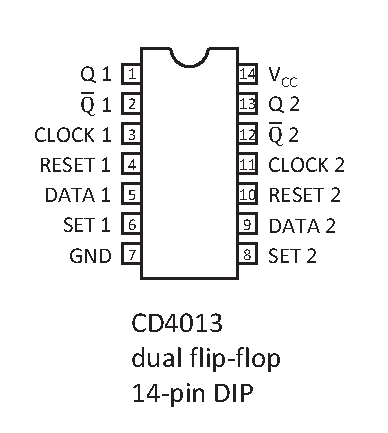
\includegraphics[scale=0.8]{appendices/pinouts/cd4013.eps}
\end{center}  

\item Start by playing with the SET and RESET inputs.  What happens to the output when you change SET to 1 (actually 5 volts)?  Does it change back when you lower SET back to 0?  What about when you do the same thing with the RESET input?

\item If the SET input is held at 1, does the RESET input have any effect on the output?  How about the reverse?

\item The SET and RESET inputs are one method of controlling the output of the flip-flop, called ``asynchronous'' operation.  You can also change the output in a ``synchronous'' mode, using a clock signal.  With the SET and RESET switches both off, set the DATA switch to 1.  Then change the CLOCK switch from 0 to 1.  At the moment the CLOCK input rises, the output should change to 1, if it wasn't there already.  What happens when you change the DATA input to 0?  Write a rule that describes what CLOCK and DATA do.

\item Does the CLOCK input have any any effect on the output when SET or RESET is held at 1?  Do SET and RESET work when the CLOCK input is held at 1?

\item {[\textit{Optional}]} Show how to use the two flip-flops on your CD4013 to wire up a set of buttons and lights that could be used to control a game show.  Two contestants are asked a question, and each contestant hits their button (a switch) as soon as they think they know the answer.  A light turns on over contestant ``A'' or ``B'' to show who buzzed in first.  After the contestant answers, the host clicks a third button to turn both lights off.  The tricky part here is that each contestant will  hit his or her button only briefly; once their hand comes off their button, the signal from the button turns off again, but you still need to hold that contestant's light on, \textit{AND} prevent the other contestant's button from having any effect---that is, until the host has reset the system for the next question.  (Hints: you can use the outputs Q or $\mathrm{\overline{Q}}$ as inputs to the system as well.  If one player's ``Q'' turns to 1, what effect should that have on the other player's controls?  You are allowed to use additional digital components like logic gates if you need to, but try to make your circuit as simple and elegant as possible.)

\end{enumerate}

